% !TEX TS-program = pdflatex
% !TEX encoding = UTF-8 Unicode

\documentclass[11pt]{article} % use larger type; default would be 10pt

\usepackage[utf8]{inputenc} % set input encoding (not needed with XeLaTeX)
\usepackage{graphicx}
\DeclareGraphicsExtensions{.pdf,.png,.jpg}

%%% Examples of Article customizations
% These packages are optional, depending whether you want the features they provide.
% See the LaTeX Companion or other references for full information.

%%% PAGE DIMENSIONS
\usepackage{geometry} % to change the page dimensions
\geometry{letterpaper} % or letterpaper (US) or a5paper or....
% \geometry{margins=2in} % for example, change the margins to 2 inches all round
% \geometry{landscape} % set up the page for landscape
%   read geometry.pdf for detailed page layout information

\usepackage{graphicx} % support the \includegraphics command and options
\usepackage[parfill]{parskip} % Activate to begin paragraphs with an empty line rather than an indent

%%% PACKAGES
\usepackage{booktabs} % for much better looking tables
\usepackage{array} % for better arrays (eg matrices) in maths
\usepackage{paralist} % very flexible & customisable lists (eg. enumerate/itemize, etc.)
\usepackage{verbatim} % adds environment for commenting out blocks of text & for better verbatim
\usepackage{subfig} % make it possible to include more than one captioned figure/table in a single float
% These packages are all incorporated in the memoir class to one degree or another...

%%% HEADERS & FOOTERS
\usepackage{fancyhdr} % This should be set AFTER setting up the page geometry
\pagestyle{fancy} % options: empty , plain , fancy
\renewcommand{\headrulewidth}{0pt} % customise the layout...
\lhead{}\chead{}\rhead{}
\lfoot{}\cfoot{\thepage}\rfoot{}

%%% SECTION TITLE APPEARANCE
\usepackage{sectsty}
\allsectionsfont{\sffamily\mdseries\upshape} % (See the fntguide.pdf for font help)
% (This matches ConTeXt defaults)

%%% ToC (table of contents) APPEARANCE
\usepackage[nottoc,notlof,notlot]{tocbibind} % Put the bibliography in the ToC
\usepackage[titles,subfigure]{tocloft} % Alter the style of the Table of Contents
\renewcommand{\cftsecfont}{\rmfamily\mdseries\upshape}
\renewcommand{\cftsecpagefont}{\rmfamily\mdseries\upshape} % No bold!

%%% END Article customizations

%%% The "real" document content comes below...

\title{Fast Track – Massively Parallel Programming Techniques Applied to Reinforcement Learning Algorithms. }
\author{Dwight Bell}
%\date{} % Activate to display a given date or no date (if empty),
         % otherwise the current date is printed 

\begin{document}
\maketitle

\section{Simple, Discrete Domains}
\subsection{Overview of the Problem}
The first problem is the N-Armed Bandit, a standard problem in reinforcement learning, described by Sutton and Barto (Sutton and Barto, 1998). The N-Armed Bandit problem gets its name from the "one-armed bandit" slot machines in casinos.  The  -armed bandit has more arms, as the name suggests.  The agent must select one of the arms, 'pull' it, and then it receives a variable reward.  The reward is based on a normal distribution that is different for each arm.  The learning problem is to determine which arm has the highest average reward by pulling arms and observing rewards.  The quality of an agent is measured as the percent of times the agent has correctly identified the highest value arm at the end of the learning period.

This problem has only one state and $n$ actions since the agent can choose one of the   arms to pull.  The agent must decide which arm to pull based on the information it has accumulated from previous rewards.  The agent needs to try all arms to get some information about each of them, but should ultimately try to concentrate on the higher-reward arms to find the best one.  The traditional single-agent approach is to keep track of the average reward produced by each arm.  The agent then decides whether to select the arm with the highest reward, or to explore the arms and choose one at random.  The learning parameter, $\epsilon$ , is used to set the probability that a random arm is chosen.  The best arm is chosen with probability $(1-\epsilon)$ .  After the training period, the arm with the highest average reward is the agent’s prediction of the best arm.

TD learning in this domain simplifies to learning $Q(a)$  since there is only one state.  The learning rate, $\alpha$ , is typically set to $1/(n+1)$ where $n$ is the number of times an action has been taken in the past.  This gives the prior estimated value of $Q(a)$ a weight of $n/(n+1)$ and the updated value equals the mean of all observed rewards for action $\alpha$.

Experiments were run using 10-, 100-, and 1000-armed bandits, with qualitatively similar results.  Results shown below are for the 100-armed bandit.

\subsection{Parallel Implementation}
In the parallel implementation for this problem the agents share their information periodically.  The processing is split between periods of learning where each agent operates independently and a sharing period where the information is consolidated from all agents and then shared.  The actual learning and sharing take place on the GPU while the CPU controls the overall process.  The high level division of activities between CPU and GPU is shown in Figure 4.  This diagram shows the basic paradigm I used for the parallel implementation of learning algorithms using the GPU.  It will be updated as the need arises as domains become more complex.

\center
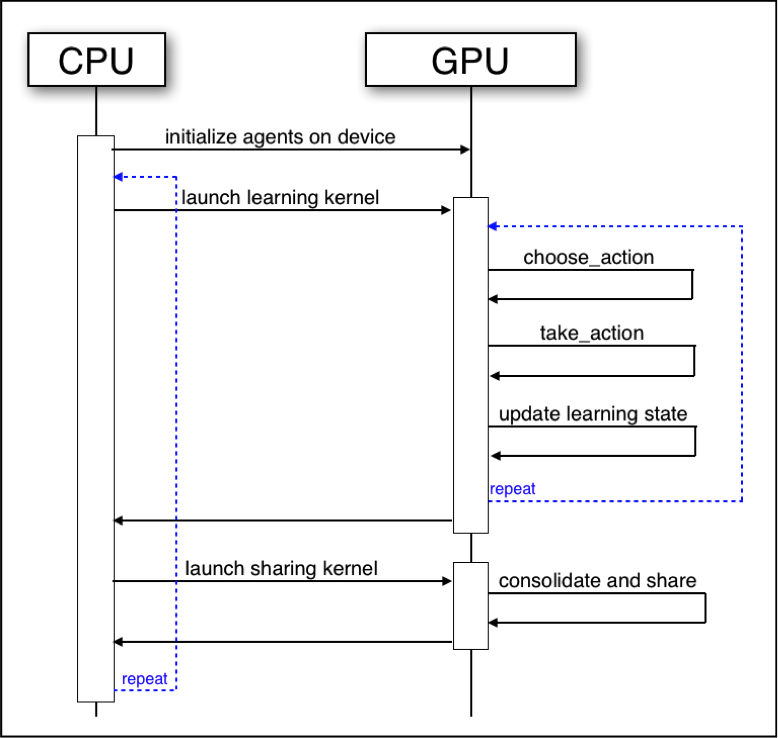
\includegraphics[scale=0.8]{fig01}
\begin{flushleft}

Key learning parameters for the multi-agent parallel approach for the  -Armed Bandit are:

\begin{itemize}
\item
The exploration probability, $\epsilon$ , same as in the single agent algorithm,
\item
the number of parallel agents, and
\item
the frequency of information sharing.
\end{itemize}

\subsection{Sharing and Differentiation}
Each agent keeps track of the number of pulls for each arm and the arm’s average payout.  When sharing occurs an overall count and average is calculated for the block of agents, and then shared back to all agents.  Let $n_i^{[j]}$ be the number of pulls stored by agent $i$ for arm $j$, and $Q_i(j)$ be the value estimated by agent $i$ for arm $j$.  The total values are calculated and each agent is updated based on the following equations for each arm $j$:

\begin{equation}
n_{total}^{[j]}=\sum_in_i^{[j]}
\end{equation}

\begin{equation}
Q_{total}(j)={ {\sum_in_i^{[j]}Q_i(j)} \over {\sum_in_i^{[j]}}}
\end{equation}

For each agent $i$:

\begin{equation}
Q_i(j) \gets Q_{total}(j)
\end{equation}

\begin{equation}
n_i^{[j]} = n_{total}^{[j]}/\mbox{\it number-of-agents}
\end{equation}

Note that in equation (???) the number of pulls stored by each agent after sharing is their share of the total number of pulls, not the total number of pulls for the entire block.  This gives less weight to the averages stored by the agent and allows those values to change more dramatically after sharing has occurred.  It also means that the sum of the number of pulls across all agents is equal to the actual total number of pulls.  This is useful when re-calculating the total values at future sharing points.  The result is that some agent's will have their average value for the best arm go down due to the random nature of rewards, perhaps causing another arm to become the best for that agent.  This has the ultimately beneficial effect of causing agents to explore other arms with high average values.

The next time sharing occurs, the block average is recalculated and quality is improved for all agents.  This gives the agents a periodic burst in learning quality at the point of sharing.  The quality may drop between sharing points as the agent’s own values are allowed to vary.  At each sharing point the quality of each agent is restored and actually improves based on the combined information.

\subsection{Results}
Experiments were run with a number of agent differentiation strategies:
\begin{itemize}
\item
partitioning the arms among the agents so when an agent was exploring it would only explore its assigned arm,
\item
random bias given to each agent used when choosing the best arm to pull,
\item
giving some agents in a group a high epsilon value so they would explore with a much greater probability than other agents, and
\item
assigning some agents to randomly choose between the top 2 or top 4 arms when selecting the best arm instead of choosing the actual best arm.
\end{itemize}

There was no dramatic improvement in learning quality from these strategies.  For some, a small improvement in learning quality was more than offset by the increased processing time to implement the more complex logic, resulting in poorer learning as a function of learning time.

Experiments were run for 10-, 100-, and 1000-armed bandits using a single agent and groups of from 4 to 8,192 parallel agents.

The results are broken down into two components to gain a better understanding of the cost and benefits of parallelization.  The first component is learning quality as a function of the number agent-time steps.  An agent time-step is one interaction between an agent and its domain, which equates to one cycle of the learning process executed by one agent.  This will measure the “parallelization penalty” which is the expected reduction in learning quality when a fixed number of agent-time steps are spread over multiple parallel agents, as compared to a single agent operating for all of the time steps.  The penalty occurs because the parallel agents operate independently and only periodically share partial information about their experience.  The single agent is expected to have better learning results, when measured on this basis, since it has complete information available at every time step.

Offsetting the parallel penalty is the speed-up in real time of the parallel implementation.  A fixed number of agent-time steps can run faster if they are executed in parallel, so for a fixed learning period, the parallel approach can execute more agent-time steps than the single agent approach.

The first experiment is for a fixed number of agent-time steps.  Learning is run for the fixed number of agent-time steps and then repeated for 1,024 trials.  Learning quality is calculated as the fraction of the 1,024 trials where the agent correctly identified the bandit with the highest expected payout, which can be determined by inspection.  Measuring learning as a function of agent-time steps gives an understanding of the algorithmic ‘parallel penalty’ from splitting up a fixed number of actions over parallel agents. The results for the 100-armed bandit are shown in Figure ??? and Figure ???.  The two graphs are the same except for the difference in agent group sizes.  Learning quality on the y-axis is measured by the probability of correctly identifying the best arm over 1,024 trials.  The blue line with circles is the result for a single agent running on the CPU and the other lines are for different numbers of parallel agents.

\end{flushleft}
\center
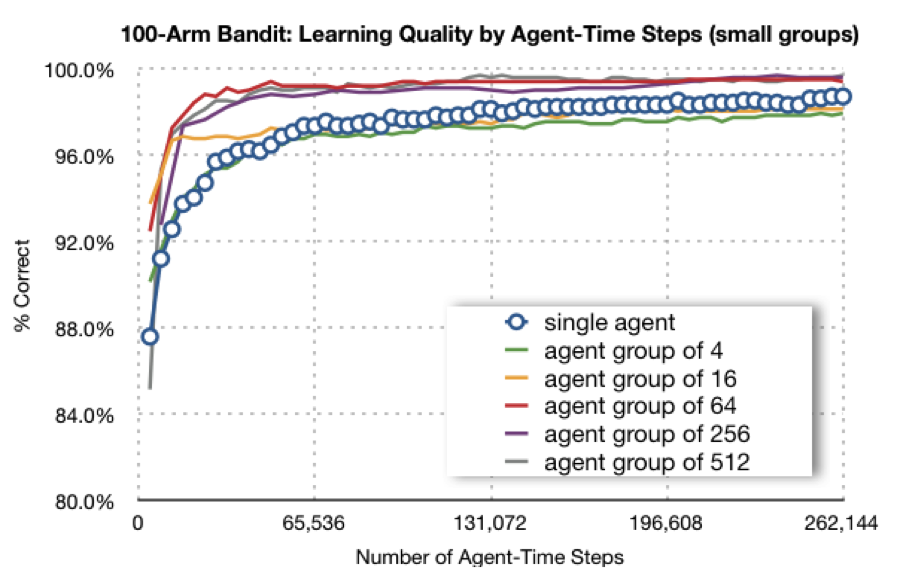
\includegraphics[scale=0.8]{fig02}
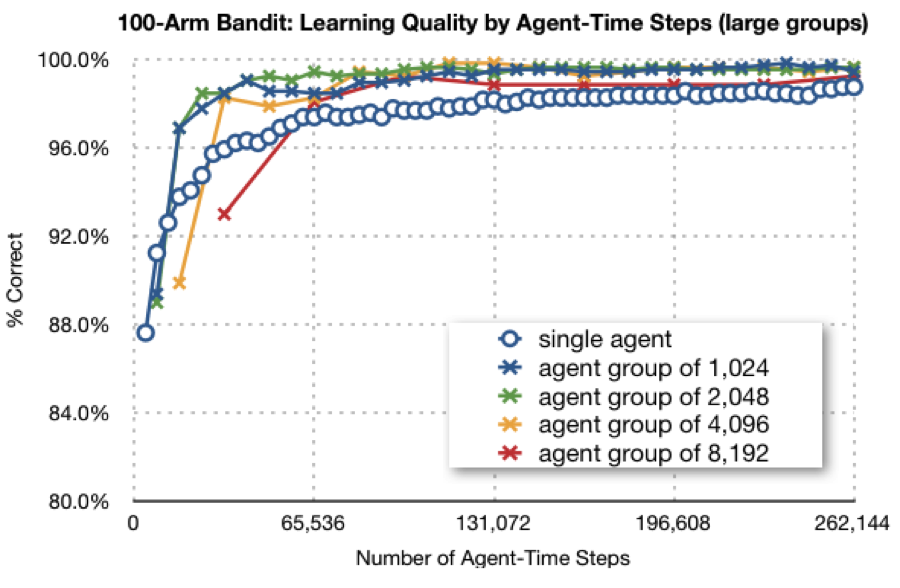
\includegraphics[scale=0.8]{fig03}
\begin{flushleft}

The results are interesting as there is no clear penalty for the parallel approach, except for agent groups of 4 or 16.  When parallel agents numbered 64 or more the parallel implementation actually produced higher quality using a fixed number of agent-time steps.  The difference appears to diminish for extremely large groups as the learning quality drops for 8,192 agents.  The multi-agent advantage is likely coming from more effective exploration due to the lack of complete information.  Each agent in the group makes an independent choice of best arm and the next action to take based on limited information, or perhaps some new unique information it has uncovered but not yet shared, leading to beneficial exploration of the state space.

The results are interesting as there is no clear penalty for the parallel approach, except for agent groups of 4 or 16.  When parallel agents numbered 64 or more the parallel implementation actually produced higher quality using a fixed number of agent-time steps.  The difference appears to diminish for extremely large groups as the learning quality drops for 8,192 agents.  The multi-agent advantage is likely coming from more effective exploration due to the lack of complete information.  Each agent in the group makes an independent choice of best arm and the next action to take based on limited information, or perhaps some new unique information it has uncovered but not yet shared, leading to beneficial exploration of the state space.

The next step is to measure learning quality as a function of learning time.  Learning time is the real elapsed time the agent spends interacting with the environment, updating its internal state, and sharing information in the case of parallel agents.  The timing values are for a single learning trial run on the CPU for a single agent, and on the GPU for parallel agents. For parallel runs, the number of time-steps is determined so that the parallel agents took at least as much time as the single agent run for 262,144 time steps.  To get credible quality measurements the results were averaged over 1024 trials for both single agent and parallel agent runs.  Learning quality as a function of learning time is shown in Figure 7.  For the two smallest numbers of parallel agents, groups of 4 or 16, the parallel implementation on the GPU did poorly compared to the single agent CPU run.  Since the time values were for a single trial, there were only 4 or 16 threads running concurrently on the GPU.  Given the complexity of the calculations and the need to frequently synchronize threads to share information, the poor results are not surprising.  For the larger numbers of parallel agents, with hundreds or thousands of threads, the parallel GPU results clearly surpass the single agent CPU results when learning quality was measured as a function of learning time.

\end{flushleft}
\center
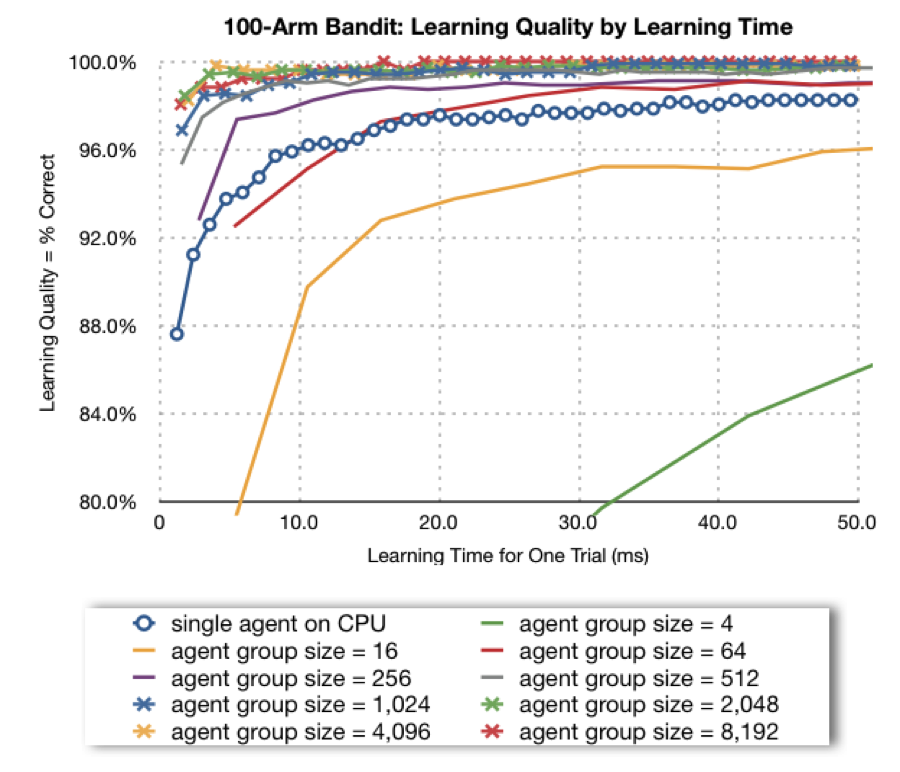
\includegraphics[scale=0.8]{fig04}
\begin{flushleft}

The last chart, Figure ???, summarizes the results of the parallel implementation of N-Armed Bandit on the GPU.  The blue bars are the learning quality for 131,072 agent-time steps.  Comparing the multi-agent blue bars to the CPU blue bar shows the improvement due to improved algorithm performance for the fixed number of agent-time steps.  The green bars are the learning quality after 37.7ms, which is the time it took to run 131,072 time steps for a single agent on the CPU.  It can be seen that with 256 or more agents, the advantage of the parallel implementation on the GPU over the single agent CPU run increased when measured as a function of time.  The drop in the fixed agent-time steps bar (blue bar) for 8,192 agents compared smaller agent groups shows that the algorithmic advantage for parallel groups does not continue to increase as group size increases.  This is also seen in Figure ???.

\end{flushleft}
\center
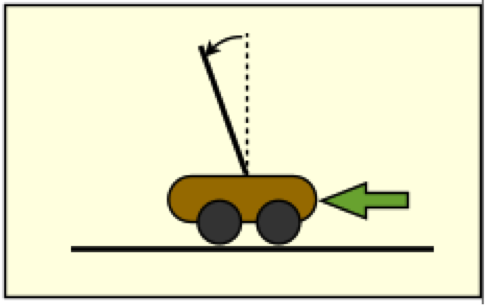
\includegraphics[scale=0.8]{fig06}
\begin{flushleft}


In summary, the massively parallel approach to the N-armed Bandit problem shows the surprising result that there is no parallel penalty for agent groups of size 64 or larger (Figure ??? and Figure ???).  Splitting a fixed number of agent-state interactions across parallel agents can actually improve the learning quality through more effective exploration.  The parallel results improved further when learning quality is measured as a function of learning time (Figure ???) as the raw speed improvement provided by the GPU allow more agent-time steps to be executed with greater speed in parallel.



\section{Simple, Continuous Domains}
\subsection{Overview of the problem}
The Pole Balancing problem, sometimes referred to as the inverted pendulum, is another canonical problem of reinforcement learning.  The paper “The Pole Balancing Problem, A Benchmark Control Theory Problem” (Brownlee, 2005) contains a detailed description of the standard definition of the problem that was used in this project.  In the Pole Balancing problem, the state consists of a cart on a track with a vertical pole attached to a hinge on the cart.  The goal is to keep the pole balanced within a certain tolerance of the vertical position and to prevent the car from going off either end of the track by applying a fixed force to either end of the car (see Figure ???).  The state of the world consists of four continuous values: the position and velocity of the cart and the angle and angular velocity of the pole.  The agent has no knowledge of how the world works and chooses between two actions: apply the fixed force to the left or to the right.

\end{flushleft}
\center
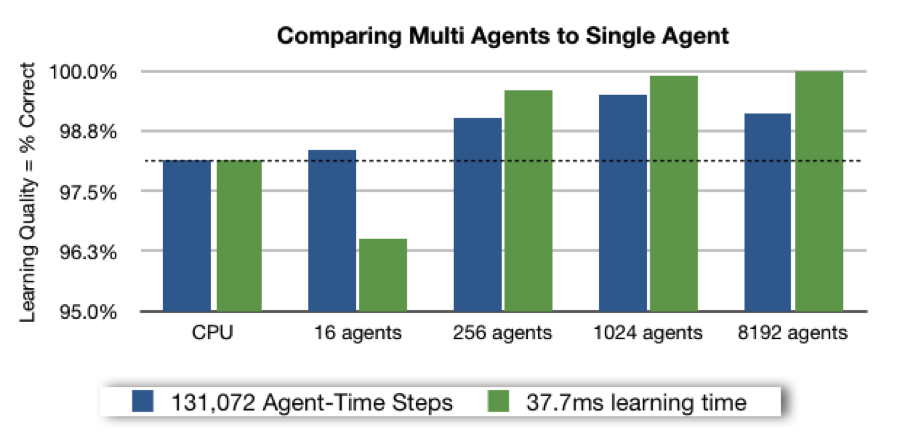
\includegraphics[scale=0.8]{fig05}
\begin{flushleft}


A reward is introduced to make this a reinforcement learning problem.  The reward is 0 for every time step that the car is on the track and the pole is in the allowable vertical range.  The agent receives a large negative reward if there is a failure due to the car running off the track, or the pole falling beyond the vertical tolerance.  Each trial begins with the state variables being initialized with random values.

This problem poses a new challenge due to the continuous state variables.  There are a number of ways that continuous variables can be handled.  One approach would be to learn a continuous function, $Q(s,a)$, over the continuous domain of the states.  This approach will be used in Chapter ??? .  For this problem we choose to partition the continuous states into a small number of cells.  The position and angle values are partitioned into 3 value ranges.  The cart velocity and angular velocity of the pole are partitioned into two value ranges, positive and negative.  This creates 36 possible discrete states of for the system.  Given the two possible actions, there are a total of 72 state-action values.  This manageable number of state-action values makes it reasonable to try to learn the $Q(s,a)$ function using TD$(\lambda)$ learning.  In this problem the agent attempts to learn the value of $Q(s,a)$ for each state-action pair using eligibility traces.  Eligibility traces should speed learning on this problem as reaching the failure state is intuitively attributable to many prior actions and not just one bad choice.

\subsection{GPU Implementation}
Temporal difference learning with eligibility traces is a complex algorithm to implement on a GPU.  Each agent must maintain a number of values for each state-action pair: the estimated $Q$-value, the eligibility trace, the weight for the $Q$-value that will be used during sharing, and the random bias amount (discussed in next section).   In addition there are random number seeds and stored values for previous state and action.  The processing within the learning GPU code is more complex than the n-Armed Bandit problem, as illustrated in Figure ???.

It is more difficult to monitor the learning process as well.  The agent’s quality cannot be determined by inspection.  It can only be determined by testing, so the learning process must be paused and the agent tested for a statistically significant number of time-steps.  For this problem learning quality is defined as the average time to failure over a trial of 8,192 time-steps.  Testing was done following each sharing phase. 

\subsection{Sharing}
Sharing among agents for this problem is done in a straightforward manner.  After a period of learning, the $Q$-values are averaged over all agents.  The average is done on a weighted basis.  Each agent maintains a weight for each state-action pair.  The weight for agent $i$ is $wgt_i(s,a)$ and it is initialized to a constant value.  During the learning process, the agent weights are updated as follows:

\begin{equation}
wgt_i(s,a) \gets wgt_i(s,a)+\alpha\epsilon_i(s,a)
\end{equation}

During sharing, an average value for all agents for $Q(s,a)$ is calculated based on the following equation:

\begin{equation}
Q_{total}(s,a)={ {\sum_iQ_i(s,a)wgt_i(s,a)} \over {\sum_iwgt_i(s,a)} }
\end{equation}

The value $Q_{total}(s,a)$ is shared with all agents and their weights are reset after sharing to the same constant initial value. 

\begin{equation}
Q_i(s,a) \gets Q_{total}(s,a)
\end{equation}

\begin{equation}
wgt_i(s,a) = \mbox{\it initial-wgt}
\end{equation}

\subsection{Differentiation}
The sharing described above produces identical agents at the start of each learning period.  Differentiation was added to the agents for this problem with beneficial results.  With differentiation, a small random bias amount is added to each agent’s $Q_i(s,a)$ values.  The amount of bias is added after sharing and it decreases over time.  The sharing update rules with differentiation are as follows, where $Rand(-1.0,1.0)$ is a uniform random number over the specified interval, {\it max-bias} is the maximum bias amount and {\it bias-decay-factor} controls the rate of reduction in the maximum bias:

\begin{equation}
Q_i(s,a) \gets Q_{total}(s,a) + Rand(-1.0,1.0) \times \mbox{\it max-bias}
\end{equation}

\begin{equation}
\mbox{\it max-bias} \gets \mbox{\it max-bias} / \mbox{\it bias-decay-factor}
\end{equation}

Randomly biasing the values of $Q(s,a)$ has the most impact on states where $Q(s,LEFT)$ is close to $Q(s,RIGHT)$, i.e. when the values learned so far do not clearly favor one action over the other.  In this situation, the random bias will cause some agents to choose $LEFT$ as the best action and others to choose $RIGHT$, generating new information about both actions from that state.  This, hopefully, leads to identifying one action as clearly the best when the agents pool their information at the next sharing point.  The next section shows the improvement in learning due to differentiation.

\subsection{Results}
Agent quality was measured for this problem as the average time to failure over 8,192 time steps.  Testing is required to determine agent quality as it cannot be determined by inspection.  Each agent is given a random starting state and runs for 8,192 time steps, noting the average time to failure during this period.  The best possible score would be 8,192, which means no failure during the testing period.  Each trial of 8,192 was repeated 1,024 times to get a statistically significant quality measurement.  Doing the quality testing on the GPU sped up the testing since the 1,024 trials can be done in parallel.

The first set of results measure the quality of learning as a function of agent-time steps.  This measurement shows the algorithmic penalty, if any, of the parallel approach.  The algorithmic penalty is the reduction in learning quality due to the fact that agents operating in parallel have less information available to them, after a given number of agent-time steps, than a single agent.  The single agent will have complete information about all actions, rewards, and state transitions, while the parallel agent must wait until a sharing point to gain any information from the experiences of the other agents.

The first graph, Figure ???, shows results by agent-time step for varying numbers of parallel agents and compares them to a single agent.  In these runs, there was no differentiation of parallel agents after sharing.  The jump in quality as agents shared information is clearly visible in the graph, but only the smaller agent groups, up to 256 parallel agents, could exceed the single agent learning quality after 262,144 agent-time steps.  The 4,096 agent group, did have an anomalous drop in learning quality at its second sharing point at 262,144 total agent-time steps.  The cause for this was not investigated and the learning quality quickly recovers when the number of time steps per agent increases, as can be seen in Figure ???.

\end{flushleft}
\center
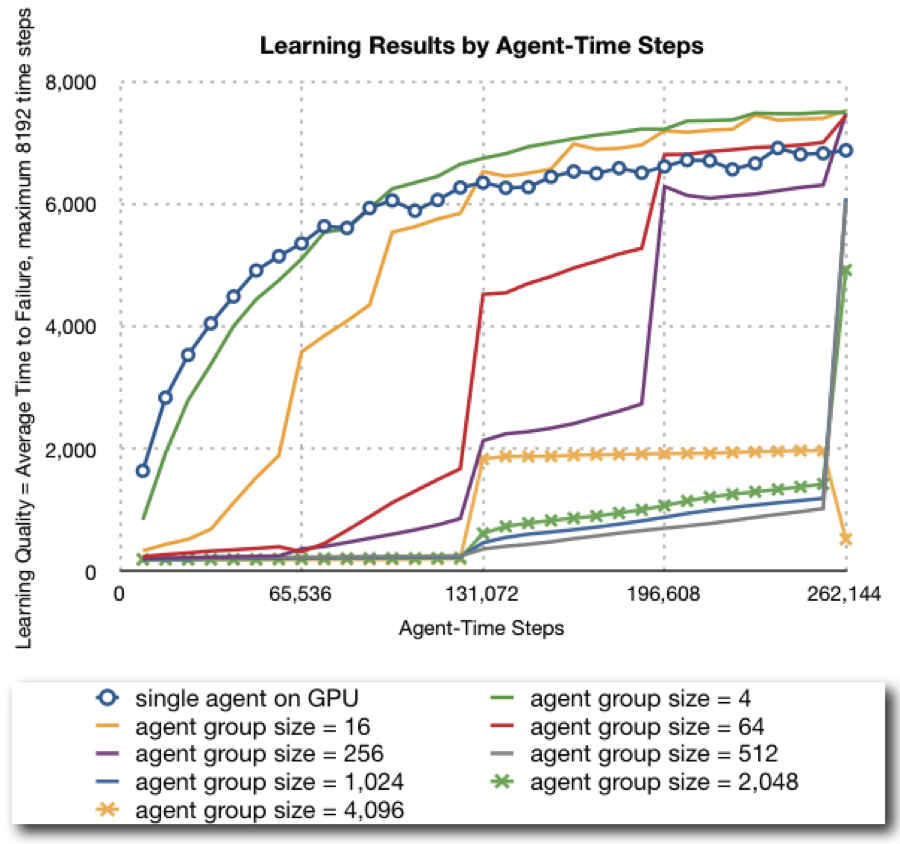
\includegraphics[scale=0.8]{fig07}
\begin{flushleft}


The frequency of sharing is a learning parameter that is determined separately by agent group size through experimentation.  As agent group size increases, the optimal number of time steps per agent between sharing decreases. 

The next measurements tested learning quality as a function of learning time.  As with the previous problem, learning time is measured based on a single run with the single agent on the CPU or group of parallel agents on the GPU.  The time spent testing the agent is, of course, excluded from the measurement.  The learning quality is then calculated by averaging the learning measurements over 1,024 trials.  The quality of learning with parallel agents is dramatically better than single agent learning for groups of 256 or larger when measured over a learning period of 400ms, as can be seen in Figure ???

\end{flushleft}
\center
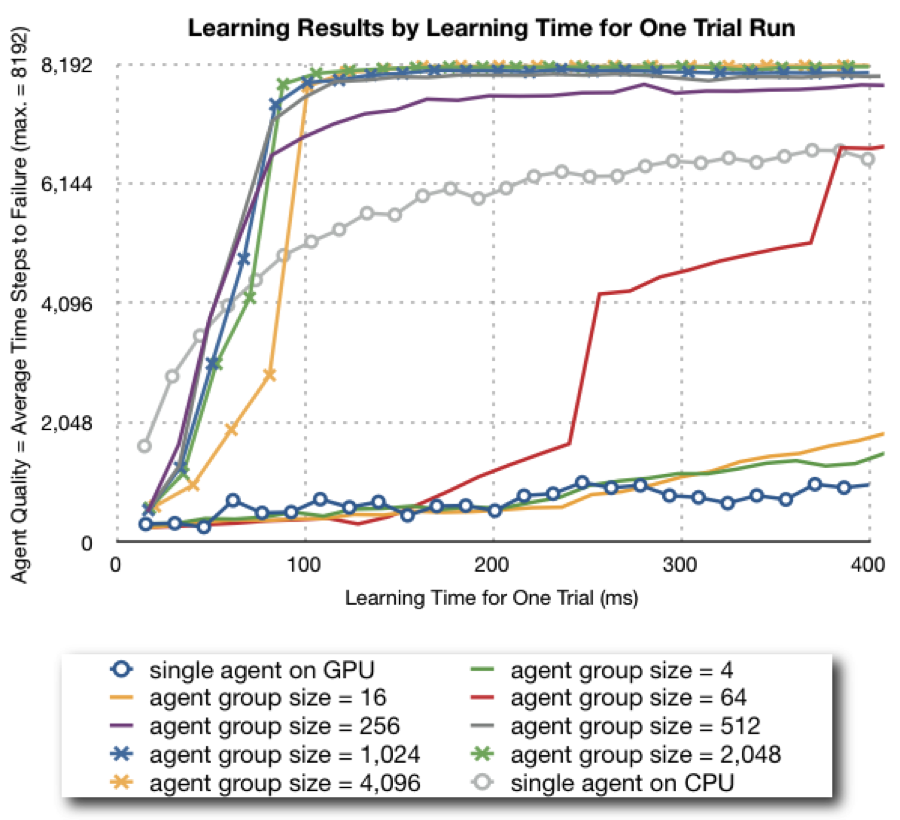
\includegraphics[scale=0.8]{fig08}
\begin{flushleft}


Agent differentiation is beneficial to parallel learning for the Pole Balancing problem, as mentioned before.  The differentiation for each agent is a small random bias added to the $Q$-values shared with each agent. The amount of random bias was determined by experimentation and decreased exponentially over time.  Differentiation dramatically improves the speed of learning for agent groups of 256 or larger.  Figure ??? shows the improvement that occurred during the first 100 ms of learning.  Ultimate quality does not change much because average quality is close to the best possible value of 8,192 and there is no room for improvement.  The final learning quality including the impact of differentiation is shown in Figure ???, clearly showing the success of the parallel approach.

\end{flushleft}
\center
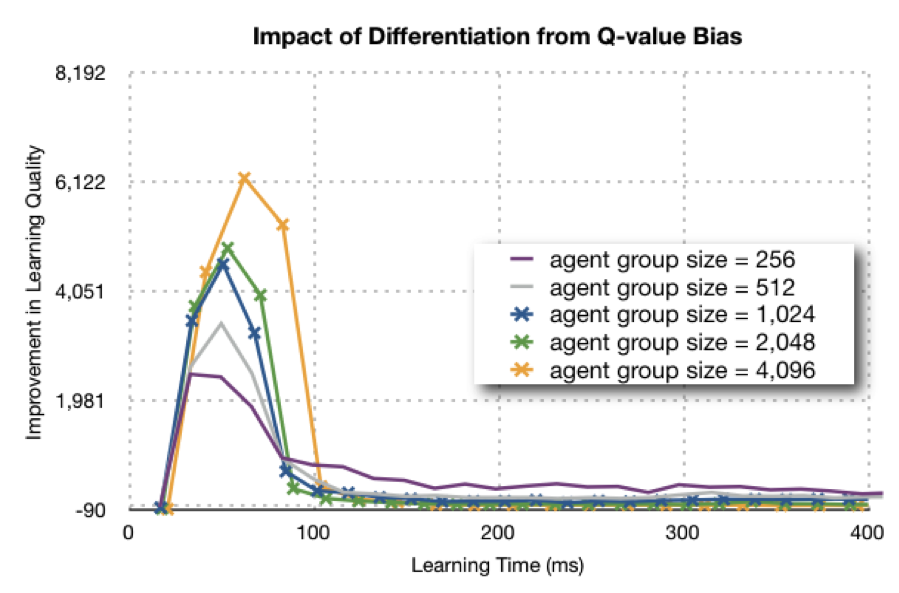
\includegraphics[scale=0.8]{fig09}
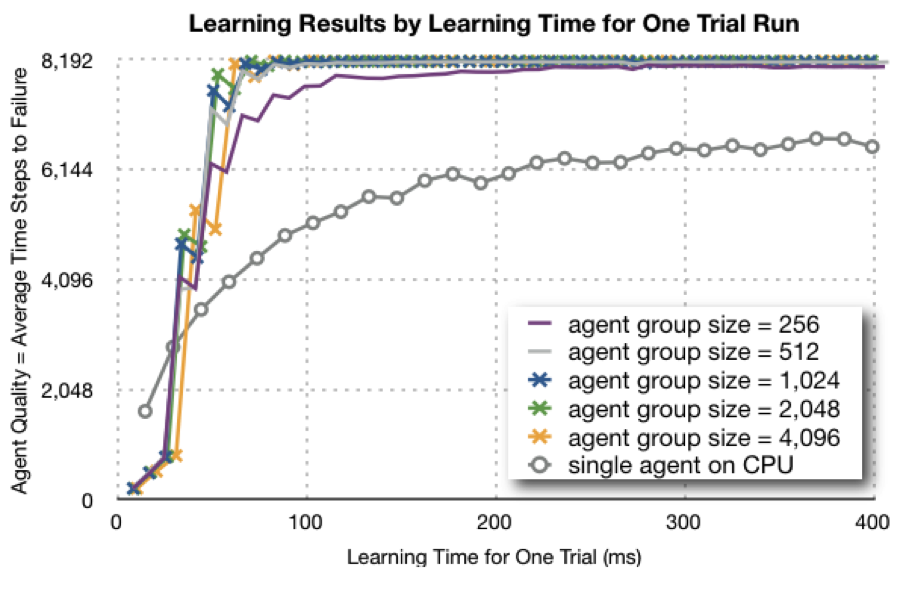
\includegraphics[scale=0.8]{fig10}
\begin{flushleft}

In summary, the massively parallel approach produces a dramatic improvement in learning quality as a function of the learning time for the Pole Balancing problem (Figure ???).  This improvement is obtained by using information sharing and agent differentiation with groups of at least 256 parallel agents. 


\section{Learning to Play a Game through Self-Play}
\subsection{Overview of the problem}
The final problem is to learn to play a game through self-play using parallel agents.  The focus is on the ultimate quality of the agent produced, with less emphasis on the speed of learning.  In this problem the agent is pre-programmed with knowledge about how the game works.  That is the agent can determine the next state of the game for any of the actions that are possible from the current state.  It also can determine which actions are legal actions from the current state.  The agent does not know the goal of the game and can not determine in advance what board positions are wins or losses, which must be learned through the reward signal.  The game uses the knight piece from chess on a 5 x 7 chessboard.  The game’s piece movement pattern, number of pieces per side, and board size are variable problem parameters but the results shown here are for knights on a 5 x 7 board and the game starts with the random placement of 5 pieces for each player.  Each player makes a move, as in chess, and a player wins if all opponent’s pieces are captured.  The game has a maximum number of turns and the result is a drawn game when that limit it is reached.

Learning through self-play was advanced by the famous work by Tesauro (Tesauro, 1994) who used TD($\lambda$) and self play to train a program to play backgammon at a master level.  This was dramatic accomplishment and has not yet been duplicated in other domains.  Tesauro points out in his work that it may be the random element that is present in backgammon that drives the learning agent into wide exploration of the state space, enabling high quality learning to take place during self-play.  The random element helps to avoid the problem of converging prematurely to a sub-optimal strategy that can happen with deterministic games.  In those games, the agent may only experience a small fraction of the state space and optimizes for this region only, since by playing itself, it never has to deal with other regions of the state space.

This game is discrete but has a large state/action space.  There are ${35 \choose 5} \times {30 \choose 5}$ possible starting positions with random placement of 5 Xs and 5 Os on a 5 by 7 board.  The total number of game states is even larger since pieces can be removed during the game.  The five knights can move in up to 8 directions each so there may be up to 40 possible actions.  Clearly, there are too many values to learn either $V(s)$ or $Q(s,a)$ for every point and generalization is required.  For this problem I chose to use a neural net to approximate the value function $V(s)$.  The value function can be used by the agent to pick optimal moves with one move look ahead.  The agent loops through possible moves, calculates the board position after each one and selects the move that results in the highest value board position.

\subsection{Neural Net Design}
The neural net must take a description of the board position and output the agent’s estimated value for that board position, $V(s)$.  I coded the board position as two series of binary values for each square on the board.  The first series had the value 1 when player X had a piece on the corresponding square and the second series indicated squares with an O piece.  A single layer of 4 hidden nodes with sigmoid activation is used and the single output node uses sigmoid activation as well.  The number of hidden nodes is a parameter that can vary.  The neural net design is shown Figure ???.

\end{flushleft}
\center
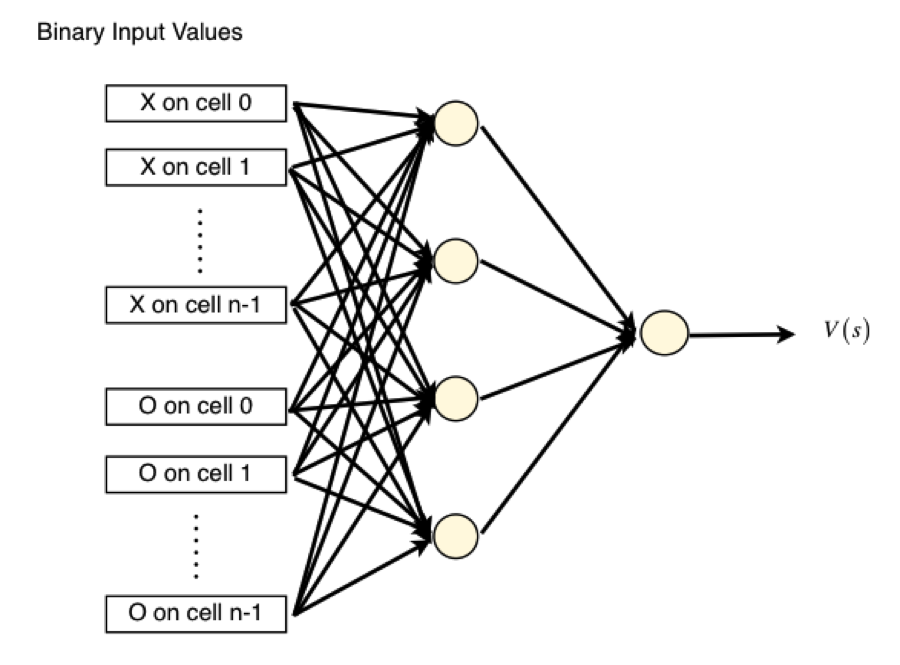
\includegraphics[scale=0.8]{fig11}
\begin{flushleft}

The learning algorithm for this problem is TD($\lambda$), building on the work done for the previous problems and adapting it to learn the $V(s)$ values.  The weight update rules combine the temporal difference equation for the value function with eligibility traces and back propagation updates for neural net weights.

The basic framework for learning is to have a group of agents learn by playing a set of games against each other.  The relative quality can be gauged by recording the agent’s winning percentage during the learning episodes.  This is shown for an 8-agent group in Figure 23.  The absolute measurement of agent quality requires some outside benchmark or test to be performed.  A benchmark opponent was used to gauge agent quality in Figure 24.  The quality measure is winning percentage calculated as $(wins + draws/2)/games$.

\end{flushleft}
\center
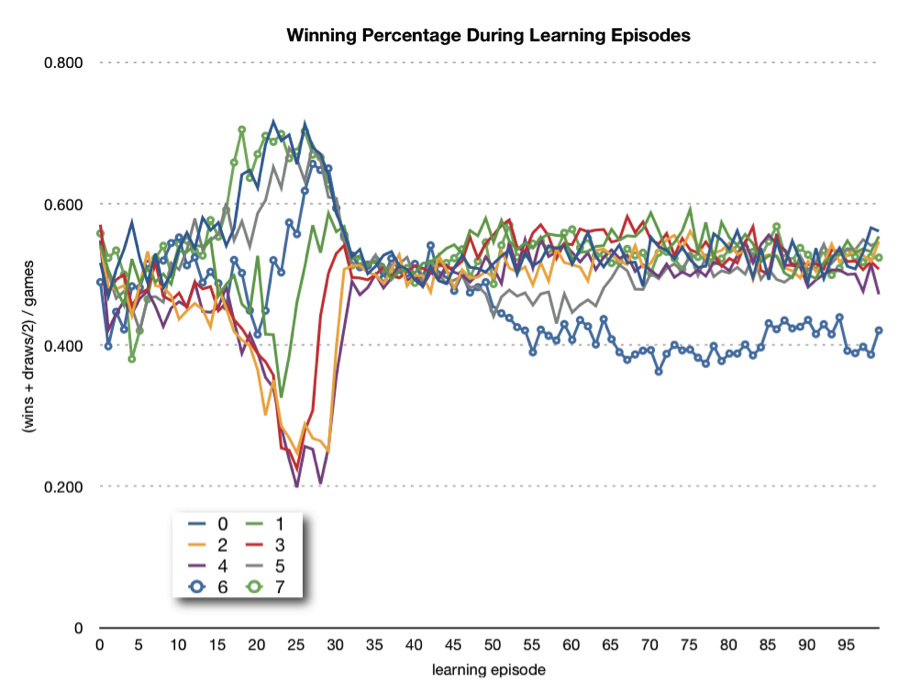
\includegraphics[scale=0.8]{fig12}
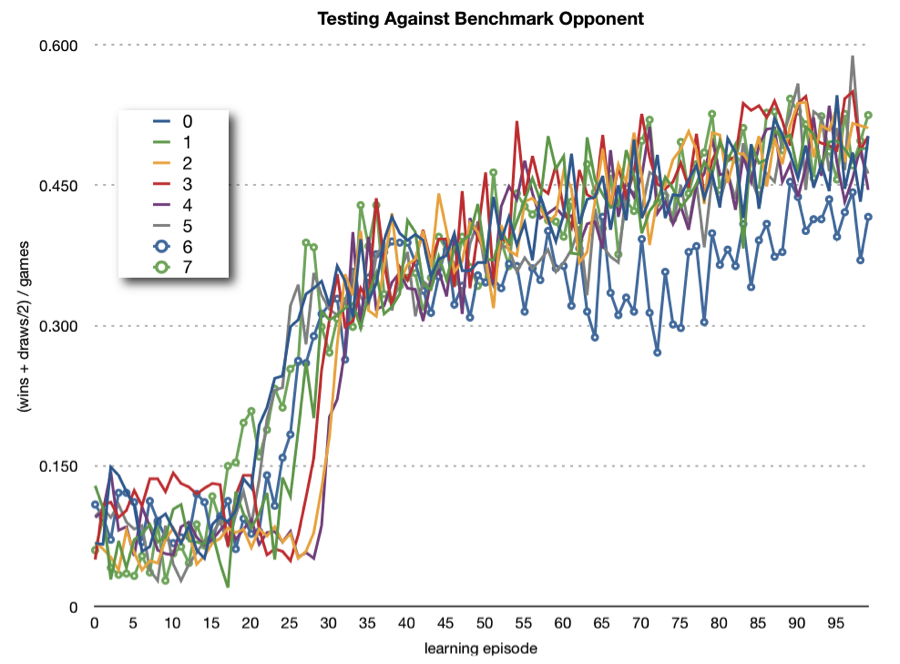
\includegraphics[scale=0.8]{fig13}
\begin{flushleft}


\subsection{GPU Implementation Issues}
The algorithm used on this problem is very compute intensive.  For each turn, the agent must look at all possible moves and estimate the value of the next board position by using the neural net estimate $V(s)$.  The GPU implementation uses multiple threads per agent to speed up the neural net calculations and to speed up the weight update calculations that are needed each turn.  Each agent has one thread per board square.  The entire group of threads within an agent will be active during some portions of the processing.  Other times, only a single thread or a smaller group of threads is needed for the calculations.  Thread activity for the choose move function is illustrated in Figure ???.  In that diagram, the green arrows represent active threads and dashed arrows are inactive threads.

\end{flushleft}
\center
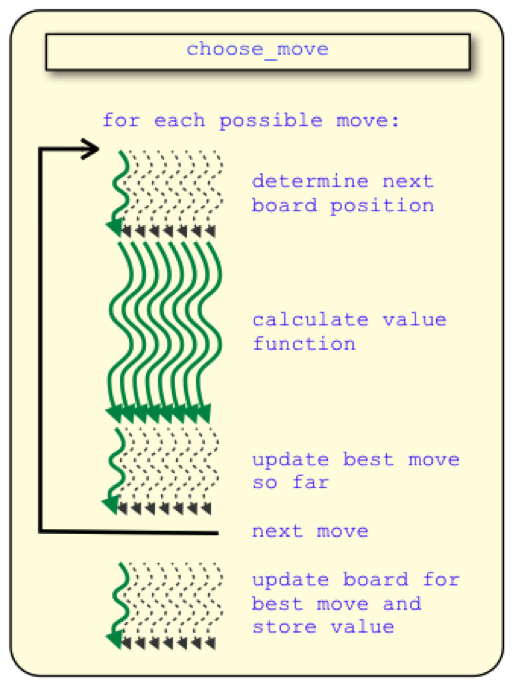
\includegraphics[scale=0.8]{fig14}
\begin{flushleft}


Agents can compete against an opponent in parallel too.  The next diagram, Figure ???, illustrates having $n$ agents compete against one opponent at the same time.

\end{flushleft}
\center
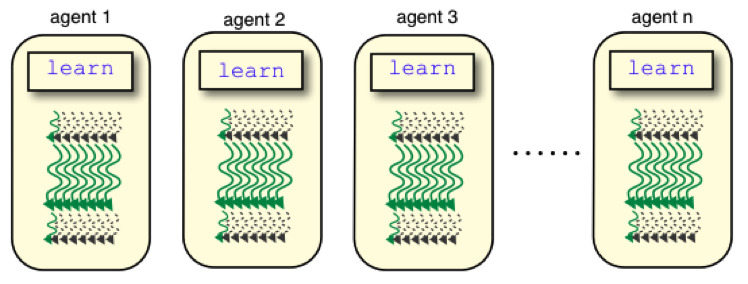
\includegraphics[scale=0.8]{fig15}
\begin{flushleft}

Having each agent compete against multiple opponents simultaneously increases parallelism further.  This approach requires creating multiple copies of the agent’s weights.  Each copy then competes against a different opponent and updates its own weights.  At the end of an episode of learning, the change in weights across all the copies of an agent is accumulated and the master copy is updated in one batch, illustrated in Figure ???.

\end{flushleft}
\center
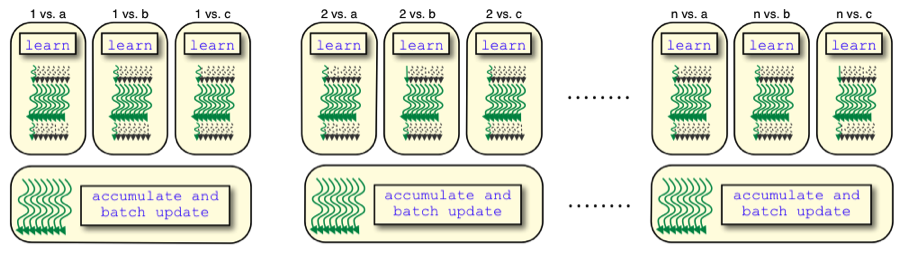
\includegraphics[scale=0.8]{fig16}
\begin{flushleft}


The processing on both the CPU and GPU is more complicated on this problem than on previous problems.  The GPU is much slower than the CPU for a single agent, but equals CPU speed with 4 agents and is faster for agent groups of 16 or more, as shown in Figure ???, which displays the learning time for one million turns.

\end{flushleft}
\center
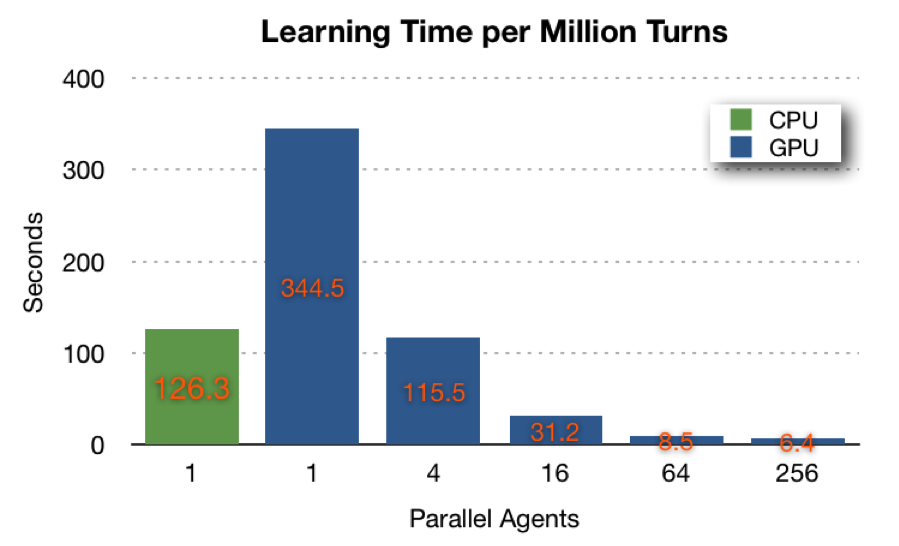
\includegraphics[scale=0.8]{fig17}
\begin{flushleft}



\subsection{Replication with Variation and Summary of Results}
There is no direct sharing between parallel agents in this problem.  Indirect sharing happens by agents competing against each other and learning.  If one agent’s quality improves, it becomes a better opponent for the other agents and the other agents should improve as a result as well.

This problem produces a wide variation of agent quality, similar to Mountain Car problem.  Selecting the best agent from a group of parallel agents, based on internal competition between agents or testing against a benchmark opponent, will improve the quality compared to the average result.  Variation in quality can be seen in Figure ???, which shows the best, worst, and average agent quality for a group of 64 parallel agents with quality measured against a benchmark opponent.

\end{flushleft}
\center
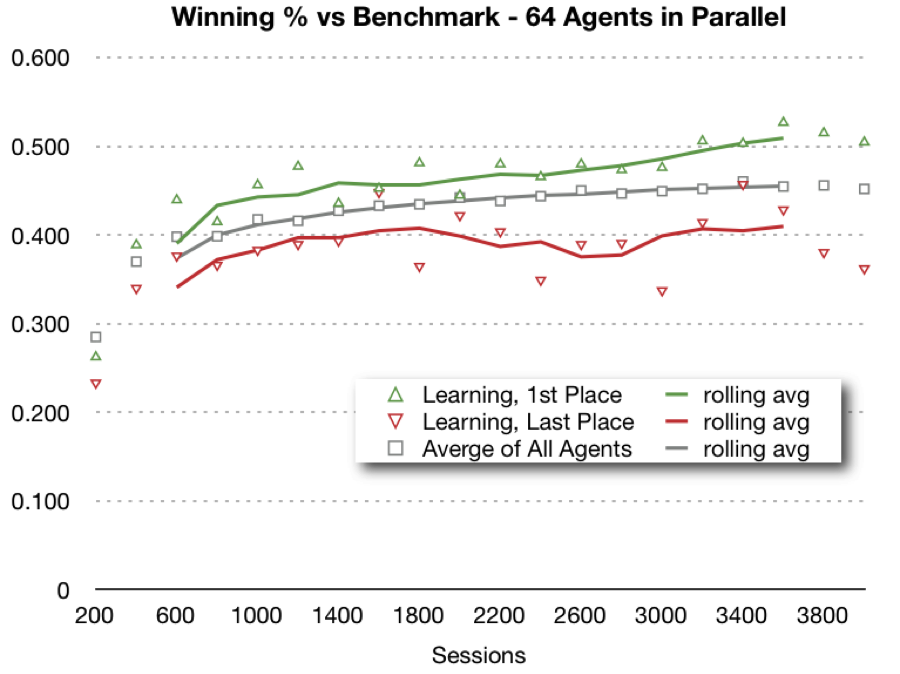
\includegraphics[scale=0.8]{fig18}
\begin{flushleft}


Another technique that works on this problem is the use of selective replication to improve the overall quality of the agent population.  After each learning episode a round-robin competition determines the relative quality of the agents.  The best agents are copied and the worst agents dropped.  In addition, this has a secondary effect of improving the opponents for all agents in the future.  Figure ??? shows the high-level sequence diagram for CPU and GPU coordination.

\end{flushleft}
\center
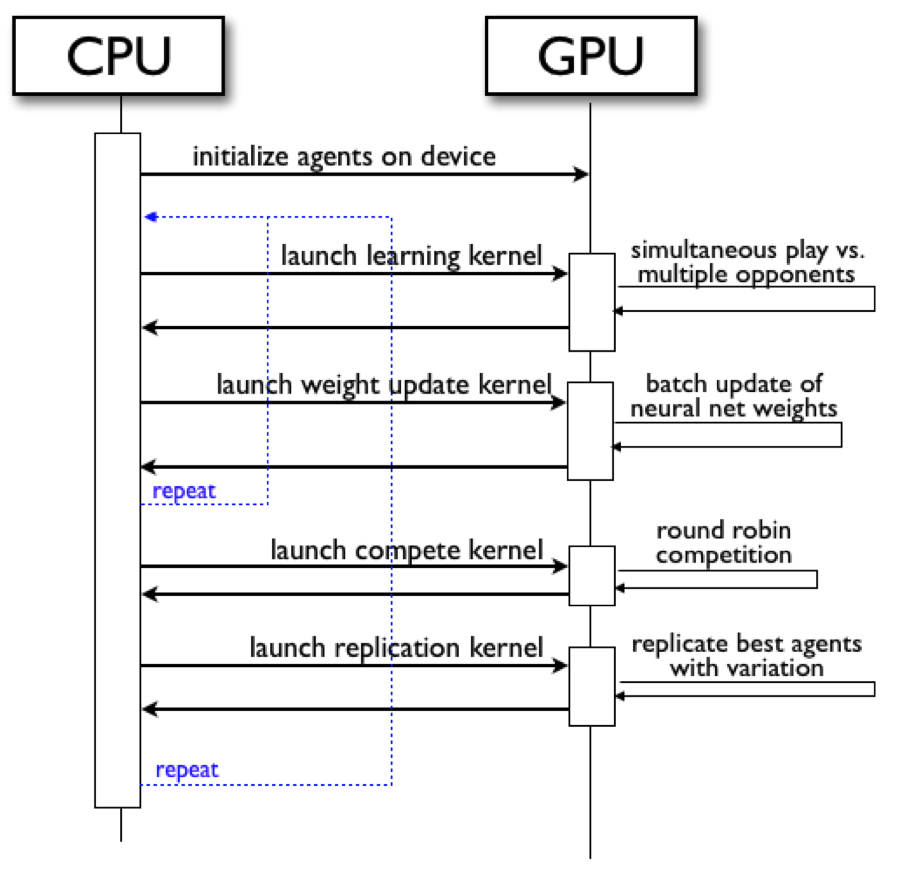
\includegraphics[scale=0.8]{fig19}
\begin{flushleft}

The replicated copies of the best agents can include some differentiation.  They can have variation in the learning parameters or slight random bias applied to the neural net weights.  Variation helped the population of agents to continue to improve over a long training session.  The last graph, Figure ???, shows the typical results when using selective replication with variation with a group of 64 agents.  

\end{flushleft}
\center
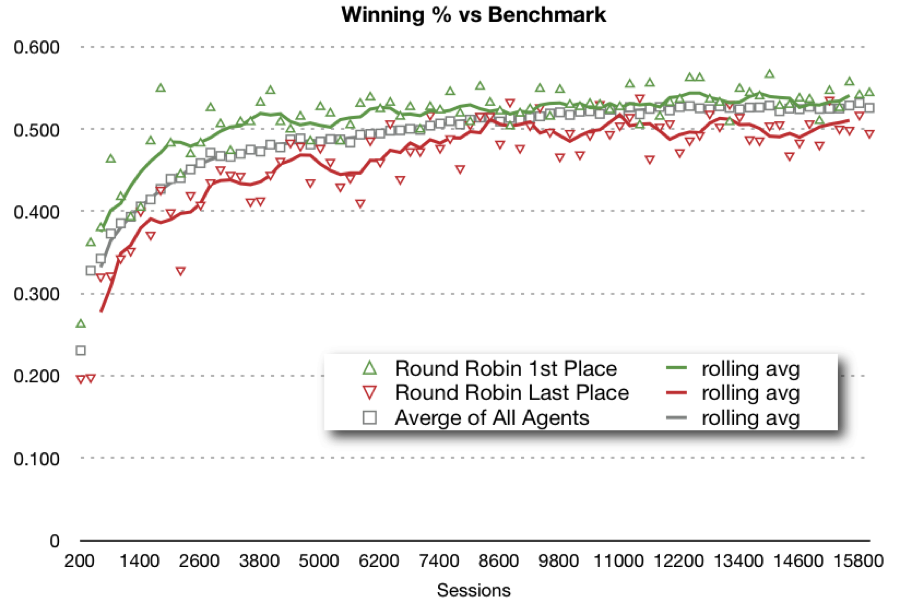
\includegraphics[scale=0.8]{fig20}
\begin{flushleft}


The parallel approach to this problem provides a variety of opponents for agents to learn from.  This can help overcome the problems with self-play using a single agent.  In addition, the evolutionary techniques of selective replication with variation allow the population of agents to continue to improve over time.

\end{flushleft}

\end{document}
